\PID \label{z:lpf_q}
\mnImportant
Функција преноса нископропусног система 
са паром конјуговано.комплесним паром полова са познатом природном учестаношћу $\upomega_{\rm N}$ 
и познатоим $Q$-фактором дат је у облику 
$H(s) = \dfrac{\upomega_{\rm N}^2 }{s^2 +  \dfrac{\upomega_{\rm N}}{Q}s + \upomega_{\rm N}^2}.$
\begin{enumerate}[label=(\alph*)]
    \item Одредити одскочни одзив датог система, $f(t)$; и 
    \item Скицирати график одзива из претходне тачке у случају када су $\upomega_{\rm N} = 1\unit{\dfrac{krad}{s}}$ и $Q = 10$. 
\end{enumerate}

\RESENJE 

(а) Одскочни одзив представља одзив на побуду $\uu(t)$ којој је у $s$-домену одговара 
$\dfrac{1}{s}$ (таблица \reft{T:LT:u}). Лапласова транформација одскочног одзива је онда 
\begin{equation}
    F(s) = \dfrac{1}{s} H(s) =
    \dfrac{\upomega_{\rm N}^2 }{ s\left( s^2 +  \dfrac{\upomega_{\rm N}}{Q}s + \upomega_{\rm N}^2 \right)}. \label{eq:\ID.F}
\end{equation}

\noindent
\begin{minipage}{\textwidth}
\begin{wrapfigure}{L}{0.2\textwidth}
    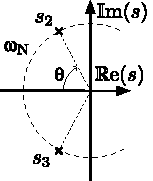
\includegraphics{fig/Q_polovi.pdf}
    \caption{Пар полова}
    \label{fig:\ID.polovi}
\end{wrapfigure}
Инверзна Лапласова трансформација одређује се растављањем на парцијалне разломке. Дати израз има три пола, 
од којих је један
$s_1 = 0$, а друга два се одређују решавањем квадратне једначине 
\begin{equation}
    s_{23} = \upsigma \pm \jj\upomega_0, \qquad \upsigma = -\dfrac{\upomega_{\rm N}}{2Q}, \qquad \upomega_0 = \upomega_{\rm N} \sqrt{1 - \dfrac{1}{4Q^2}} 
\end{equation}
За тако одређени пар комплексно конјугованих полова може се приметити да се они налазе на кружници полупречника $\upomega_{\rm N}$, а заклапају угао 
$\arccos\left(\dfrac{1}{2Q}\right)$ са негативним делом реалне осе, као што је илустровано на слици \ref{fig:\ID.polovi}. 
Пар полова је комплексно конјугован у случају када је $Q > 1/2$, иначе су полови реални.
\end{minipage} \\[5mm]
%

\noindent 
Растављањем на парцијалне разломке израза \eqref{eq:\ID.F} према додатку \ref{a:pfd} се онда добија облик 
\begin{equation}
    F(s) = \dfrac{A}{s} + \dfrac{B}{s - (\upsigma + \jj\upomega)} + \dfrac{B^\ast}{s - (\upsigma - \jj\upomega)},
\end{equation}
где се коефицијенти налазе методом из истог додатка 
\begin{eqnarray}
    A &=& \dfrac{\upomega_{\rm N}^2}{ \xcancel{s}\left( s^2 +  \dfrac{\upomega_{\rm N}}{Q}s + \upomega_{\rm N}^2 \right)} \Biggr|_{s = 0} = 1 \\
    B &=&  \dfrac{\upomega_{\rm N}^2}{ s \jj 2 \upomega_0 } \Biggr|_{s = \upsigma + \jj\upomega_0} = -\jj \dfrac{\upomega_{\rm N}^2}{2 \upomega_0 (\upsigma + \jj\upomega)}
\end{eqnarray}
Применом одговарајуће табличне трансформације \reft{T:LT:u} и општег резултата задатка \ref{z:damp_sin}, одређује се одзив у временском домену
\begin{eqnarray}
    f(t) &=& 
    \underbrace{
    \ILT{\dfrac{1}{s}}
    }_{\reft{T:LT:u}: \uu(t)}
    + 
    \underbrace{
    \ILT{
        \dfrac{B}{s - (\upsigma + \jj\upomega)} + \dfrac{B^\ast}{s - (\upsigma - \jj\upomega_0)}
    }}_{ \text{Задатак \ref{z:damp_sin}: } 2|B| \cos(\omega_0 t + \arg B)\uu(t)  } \label{eq:\ID.oblik_resenja}
    % \\
    % &=&
    % \left(
    % 1 
    % +
    % \dfrac{\upomega_{\rm N}}{\upomega_0} \cos\left(
    %     \upomega_0 t + 
    % \right)
    % \right) 
\end{eqnarray}
Са тим у виду, одредимо модул и аргумент коефицијента $B$ према\footnote{Користе се идентитети комплексних бројева $|uv| = |u| \cdot |v|$, и 
$\arg(u/v) = \arg(u) - \arg(v)$. }
\begin{eqnarray}
    |B| &=& \left| -\jj \dfrac{\upomega_{\rm N}^2}{2 \upomega_0 (\upsigma + \jj\upomega_0)} \right|
    = \dfrac{\upomega_{\rm N}}{2\upomega_0 \underbrace{|\upsigma + \jj\upomega_0|}_{\mathclap{=\upomega_{\rm N}, \text{Слика \ref{fig:\ID.polovi}}}}}
    = \dfrac{\upomega_{\rm N}}{2\upomega_0} = \dfrac{1}{2 \sqrt{1 - \frac{1}{4Q^2}} }
    \\ 
    \arg B &=& \arg \left( 
        -\jj \dfrac{\upomega_{\rm N}^2}{2 \upomega_0 (\upsigma + \jj\upomega_0)} 
    \right)
    = \arg(-\jj) - \arg(\upsigma + \jj\upomega_0) = -\dfrac{\uppi}{2} - \arctan\left( \dfrac{\upomega_0 }{\upsigma} \right) \\
    &=& - \dfrac{\uppi}{2} + \arctan \left( \sqrt{4Q^2 - 1} \right)
\end{eqnarray}
Користећи и идентитет да је $\cos(x - \uppi/2) = \sin(x)$, заменом добијених вредности у \eqref{eq:\ID.oblik_resenja} добија се коначни облик 
\begin{equation}
    f(t) = \left(
        1 -
        \dfrac{1}{\sqrt{1 - \frac{1}{4Q^2}} }
        \ee^{\upsigma t}
        \sin\left(
            \upomega_0 t + \arctan (\sqrt{4Q^2 - 1})
        \right)
    \right) \uu(t). \label{eq:\ID.resenje_final}
\end{equation}

(б) За скицирање одзива може се апроксимирати $\sqrt{4Q^2 + 1} \approx 2Q$, па је 
$\arctan(\sqrt{4Q^2 + 1}) \approx \arctan 20 \approx \uppi/2$. За члан који се односи на амплитуду је на сличан начин 
$
\dfrac{1}{\sqrt{1 - \frac{1}{4Q^2}} } \approx 1
$. Кружна фреквенција простопериодичног дела је такође $\upomega_{\rm 0} \approx \upomega_{\rm N}$, док је 
$\upsigma = -\dfrac{\upomega_{\rm N}}{2Q} = 50\unit{s^{-1}}$. Заменом свега добијеног има се 
$
    f(t) \approx \left(
        1 - \ee^{- 50\unit{s^{-1}} t } \cos \left( 1\unit{\dfrac{krad}{s}} t \right)
    \right) \uu(t),
$ чији је график приказан на слици \ref{fig:\ID.odziv}. На слции се може уочити појава осцилација у одзиву филтра које су  
последица полова у близини имагинарне осе комплексне равни. $Q$-фактор претежно утиче на брзину ишчезавања ових осцилација, 
док је фреквенција осциловања практично једнака природној учестности $\upomega_{\rm N}$. 
\begin{figure}[ht!]
    \centering
    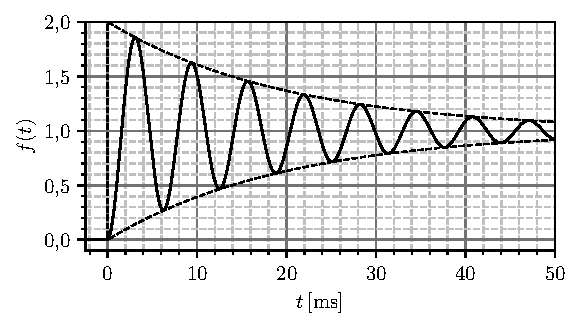
\includegraphics{fig/Q_odziv.pdf}
    \caption{Тражени одскочни одзив, анвелопа синусоиде приказана је испрекидано, 
    $1 \pm \ee^{\upsigma t}$.}
    \label{fig:\ID.odziv}
\end{figure}

На слици \ref{fig:\ID.comment} приказани су оскочни одзиви решења \eqref{eq:\ID.resenje_final} за различите 
вредности $Q$-фактора и природних учестаности полова. Повећање $Q$-фактора доводи до израженијих
осцилација у одзиву (тзв. \textit{ringing}), што указује на смањену стабилност система. Мера стабилности 
је непосредно повезана са положајем полова у комплексној равни: што су они ближи граници стабилности, систем је мање 
стабилан. Такав приступ омогућава квантитивну оцену стабилности, која је основа разних критеријума стабилности.
\begin{figure}[ht!]
    \centering
    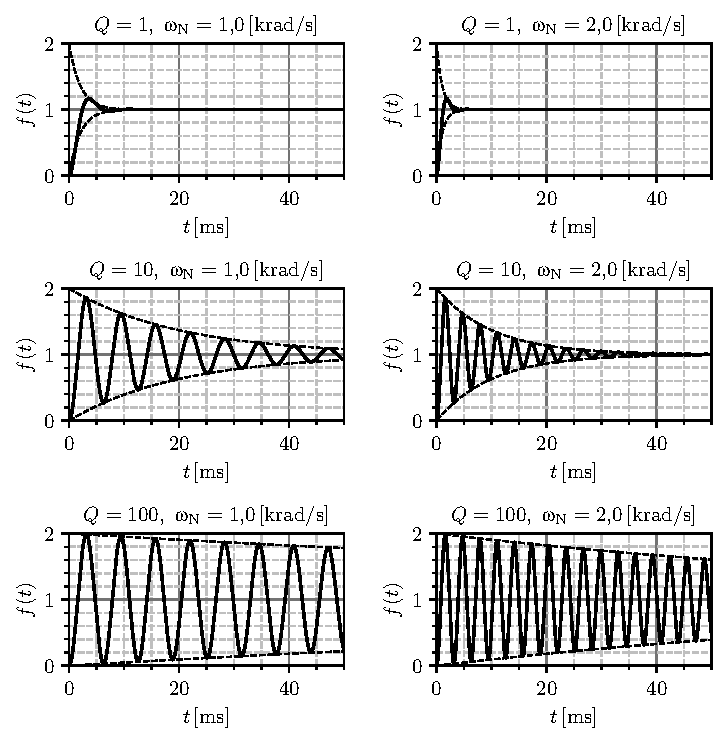
\includegraphics[scale=1]{fig/Q_razliciti_odzivi.pdf}
    \caption{Уз коментар. Утицај $Q$-фактора и природне учестаности на одскочни одзив нископропусног система 
    другог реда}
    \label{fig:\ID.comment}
\end{figure}
